\section{Dispersion}
\label{sec:Dispersion}

The goal of a swarm dispersion algorithm is to achieve positional configurations that satisfy some user-defined criteria.  Such criteria include distances from neighboring agents, densities of neighboring agents, or the total area covered by the entire swarm.  Practical applications of dispersion algorithms for mobile agents include: conducting a search of the Martian landscape using biologically-inspired tumbleweed robots \cite{kolacinski:SwarmRovers}, forming an ad-hoc wireless network using autonomous UAVs or blimps \cite{brown:AdHocUAV}, or as a preparatory action for a more complex swarm algorithm.  The key to the dispersion algorithm is a measure of the quality of an agent's position. The measure used in this demonstration is a binary function, returning true if the agent's position is good and false if the position is bad, where good and bad are defined relative to the number of neighbors for a given agent.  \refAlgorithm{SimpleDispersion} provides a pseudo-code description of the dispersion algorithm.

\begin{algorithm}[ht]
\caption{Simple dispersion}
\label{alg:SimpleDispersion}
	\begin{algorithmic}[1]
		\IF{Evaluate(pos) == Unsatisfied}
			\STATE Move randomly
		\ELSE
			\STATE Do not move
		\ENDIF
	\end{algorithmic}
\end{algorithm}

\begin{figure}[ht]
	\centering
	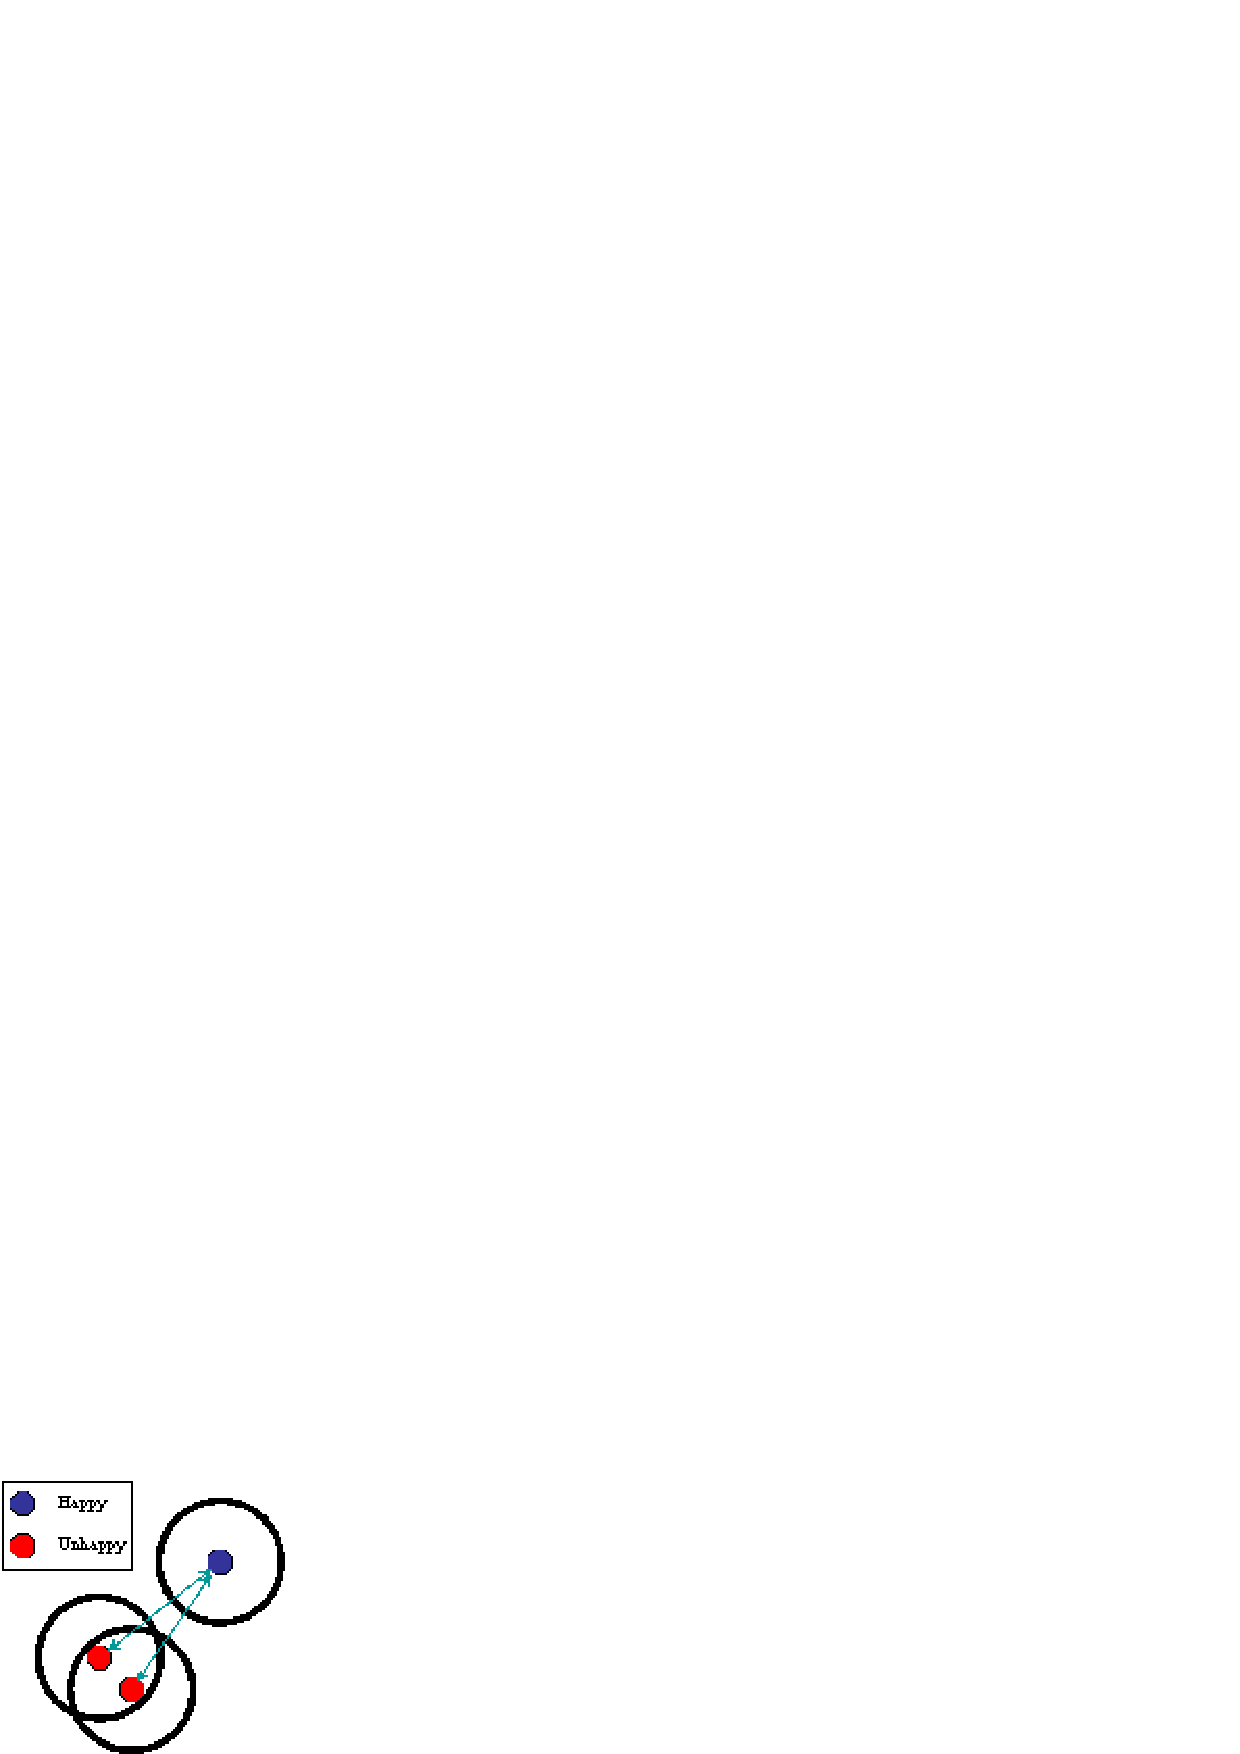
\includegraphics[scale=.65]{Figures/DispersionExample.jpg}
\label{fig:DispersionExample}
\caption{An example of the dispersion algorithm in action}
\end{figure}

The goal of each agent is to achieve and maintain a constant minimum and maximum distance from all neighboring agents.  \refFigure{DispersionExample} shows the basic situations that will arise during the execution of a dispersion algorithm.  As shown in the figure, an agent can have unsatisfied positional constraints if they are either too close or too far from other agents.  An agent's constraints will only be satisfied when none of their neighbors are too far away or too close.  To better illustrate the aggregate behavior of the dispersion algorithm, a simulation with 125 agents on a $100 \times 100$ grid environment was performed.   \refFigure{DispersionBeforeAfter} shows the initial and final swarm configurations of the simulation.  

\begin{figure}[ht]
	\centering
	\subfigure[Initial configuration before executing the dispersion algorithm]
	{
		\includegraphics[width=.45\textwidth]{Figures/DispersionInitial.jpg}
		%\includegraphics[width=.45\textwidth]{Figures/Tumble1.jpg}
		\label{fig:DispersionBefore}
	}
	\qquad	
	\subfigure[Final configuration after executing the dispersion algorithm]
	{
		%\includegraphics[width=.45\textwidth]{Figures/DispersionFinal.jpg}
		\includegraphics[width=.45\textwidth]{Figures/Tumble4.jpg}
		\label{fig:DispersionAfter}
	}\\
	
\caption[A 125 agent swarm executing the dispersion algorithm.]{The initial and final configurations of a 125 agent swarm executing the dispersion algorithm on a $100 \times 100$ region.}
\label{fig:DispersionBeforeAfter}
\end{figure}

%The red agents are not satisfied with their position because they are too close to each other, and thus are mutually violating the minimum distance constraints.  The blue agent is satisfied with its position because the red agents are being kept at a distance that satisfies both the minimum and maximum distance requirements.

\refTable{SweepDispersionParameters} is a summary of the simulation parameters used in implementing the dispersion algorithm.  Assume a swarm is randomly spread throughout a region, with the goal of dispersing out to a certain density in order to provide a predetermined level of area coverage.  The goal of each agent is to achieve a position where no neighboring agent is within 2 grid units, and there is at least one agent within 5 grid units.  Each agent is equipped with a distance sensor that can determine the distance of neighboring agents who are within 6 grid units.  

\begin{table}[ht]
\begin{center}
  \begin{tabular}{|l|p{6cm}|}
    \hline
    \textbf{Number of Agents} & 100 \\
    \hline
    \textbf{Size of Region} & $20\times20$, $30\times30$, $50\times50$ \\
    \hline
    \textbf{Actions} & Move-RANDOM, Move-NONE \\
    \hline
    \textbf{Sensors} & Neighbor-Distance \\
    \hline
    \textbf{Dispersion Measure} & No agents closer than 2 grid units and at least 1 agent within 5 grid units \\
    \hline
  \end{tabular}
  \caption{Summary of dispersion simulation parameters}
  \label{tab:SweepDispersionParameters}
\end{center}
\end{table}

For each region size, 50 simulations were run using different random initial positions for each trial.  The region boundaries provide an upper limit on the total area covered by the swarm, thus region size can indirectly influence execution speed.  In the $50\times50$ case, on average the swarm disperses to a stable pattern within 300 time steps.  The $30\times30$ case takes substantially longer to emerge a stable pattern, usually around 500--600 time steps due to the reduced amount of area with which to disperse.  Some simulations in the $30\times30$ case took over 1000 time steps to settle into a stable pattern due to clusters of agents forming in a corner of the region, thus reducing the number of useful moves available.  Finally, the $20\times20$ case magnifies the clustering problem seen in the $30\times30$ case as the agents themselves occupy one-quarter of the available region space.  A stable dispersion pattern, one where all agents simultaneously satisfy their positional constraints, is not found by the swarm in any of the $20\times20$ trials.  As an experiment, several of the $20\times20$ simulations were allowed to run for over 2000 time steps in an attempt to find a stable dispersion.  Though no stable dispersions are achieved, non-stabilizing dispersion patterns do begin to emerge.  A non-stabilizing dispersion can be thought of as the case where on average the swarm is satisfying the aggregate positional constraints, but cannot satisfy each agent's individual constraints due to other factors, such as the size of the region.


